\documentclass[12pt,oneside,final]{ucthesisucsbmath2010}
\usepackage{amsthm}
\usepackage{amsmath}
\usepackage{amssymb}
\usepackage{latexsym}
\usepackage{bbm}
%\usepackage[pdftex]{graphicx,color}
\usepackage[dvips]{graphicx}
\usepackage{enumerate}
\usepackage{verbatim}
\usepackage{amsfonts}
\usepackage{epsfig}
\usepackage{tikz}
\usetikzlibrary{fit}
\usetikzlibrary{shapes}
%\usepackage{mathdots}
\usepackage{url}
%\usepackage{subfigure}
\usepackage{float}
\usepackage{mathtools}
%\usepackage{algorithm2e}
%\usepackage{algpseudocode}
\usepackage{algorithm}
\usepackage{algorithmic}
\usepackage{caption}
\DeclareGraphicsRule{*}{mps}{*}{}

\renewcommand{\algorithmicrequire}{\textbf{Input:}}
\renewcommand{\algorithmicensure}{\textbf{Output:}}
\newcommand{\nl} {\newline}
\newcommand{\normal}{\triangleleft}
\newcommand{\union}{\bigcup}
\newcommand{\intersect}{\bigcap}
\newcommand{\QED}{\blacksquare}
\newcommand{\homo}{\simeq}
\newcommand{\A}{\big(A_1,\ldots,A_m\big)}
\newcommand{\R}{\mathbb{R}}
\newcommand{\Z}{\mathbb{Z}}
\newcommand{\Q}{\mathbb{Q}}
\newcommand{\N}{\mathbb{N}}
\newcommand{\C}{\mathbb{C}}
\newcommand{\h}{\mathbb{H}}
\newcommand{\T}{\mathcal{T}}
\newcommand{\s}{\mathcal{S}}
\newcommand{\E}{\mathcal{E}}
\newcommand{\F}{\mathcal{F}}
\newcommand{\p}{\mathcal{P}}
\newcommand{\w}{\mathcal{W}}
\newcommand{\ov}{\overline}
\newcommand{\comp}{\overline}
\newcommand{\snd}{\Sigma_{n,d}}
\newcommand{\pnd}{\R[x_1,\ldots,x_n]_{2d}}
\newcommand{\pn}{\R[x_1,\ldots,x_n]}

\DeclareMathOperator{\trace}{trace}
\DeclareMathOperator{\kernel}{ker}
\DeclareMathOperator{\conv}{conv}
\DeclareMathOperator{\rank}{rank}
\DeclareMathOperator{\co}{co}

\newcounter{qcounter}

\newtheorem{thm}{Theorem}[section]
\newtheorem{prop}[thm]{Proposition}
\newtheorem{lem}[thm]{Lemma}
\newtheorem{cor}[thm]{Corollary}
\newtheorem{conj}[thm]{Conjecture}

\theoremstyle{definition}
\newtheorem{defn}[thm]{Definition}
\newtheorem{nota}[thm]{Notation}
\newtheorem{tech}[thm]{Technique}
\newtheorem{examp}[thm]{Example}

\includeonly{background}

\begin{document}

				%%%%TITLE PAGE%%%%
\title {Quadratic Convexity and Sums of Squares}
\author{Martin Ames Harrison}
\report{Dissertation}
\degreemonth{December}
\degreeyear{2013}
\approvalmonth{October}
\approvalyear{2013}
%\degreesemester{Spring}
\degree{Doctor of Philosophy}
\chair{Professor Mihai Putinar}
\committeeII{Professor Carlos Javier Garcia-Cervera}
\committeeIII{Professor Kenneth Ralph Goodearl}
\nummembers{3}
%\othermembers{cte 1\\
%cte 2}
%\numberofmembers{3}
\prevdegrees{BS California Polytechnic State University, San Luis Obispo 2007\\
MA University of California, Santa Barbara 2013}
\field{Mathematics}
\campus{Santa Barbara}
\maketitle

				%%%%SIGNATURE AND COPYRIGHT PAGES%%%%
\begin{frontmatter}
\approvalpage
\copyrightpage

				%%%%DEDICATION%%%%
%\begin{dedication}
%\center{For Rich}
%\end{dedication}

				%%%%ACKNOWLEDGEMENTS%%%%
\begin{acknowledgements}
I thank Professor Mihai Putinar for the guidance and encouragement he has provided me over the last five years. I thank my committee members Professor Carlos Garcia-Cervera and Professor Ken Goodearl for several helpful discussions. I thank Medina Price for her inexhaustible patience and empathy. Finally, I thank Akshat Kumar for doing mathematics with me.
\end{acknowledgements}

				%%%%CV%%%%
\begin{vitae}
\begin{vitaesection}{Education}
BS, Mathematics, California Polytechnic State University-San Luis Obispo, 2007\\
MA, Mathematics, University of California-Santa Barbara, 2009\\
PhD, Mathematics, University of California-Santa Barbara, 2013 (expected)
\end{vitaesection}\
\begin{vitaesection}{Positions}
Teaching Assistant, University of California-Santa Barbara, 2007-2013\\
Teaching Associate, University of California-Santa Barbara, Summer 2009
\end{vitaesection}\
\begin{vitaesection}{Publication}
``Pfister's Theorem Fails in the Free Case", \emph{Mathematical Methods in Systems, Optimization and Control}, pp. 189-194, Birkh\"{a}user Basel, 2012.
\end{vitaesection}\
\begin{vitaesection}{Fields of Study}
Functional Analysis and Convex Geometry\\
Advisor: Mihai Putinar
\end{vitaesection}

\end{vitae}

				%%%%ABSTRACT%%%%
\begin{abstract}
The \emph{length} of a sum of squares $\sigma$ in a ring $R$ is the smallest natural $k$ such that $\sigma$ can be realized as a sum of $k$ squares in $R$. For a set $S\subseteq R$, the \emph{pythagoras number} of $S$, denoted by $\p(S)$, is the maximum value of length over all $\sigma \in S$. This dissertation is motivated by the following simple question: if $R=\pn$ and $S=\pnd$ (the span of forms of degree $2d$), then what is $\p(S)$?

By parametrizing the set of sums of $k$ squares, we obtain a new formulation of the problem: when is the image $A(\R^N)$ of a quadratic map $A:\R^N \to \R^M$ convex? We prove several results on the structure of quadratic images and of the set of quadratic maps in general. In particular, we give conditions under which convexity of $A(\R^N)$ is equivalent to convexity of its compact intersection with an affine hyperplane. We prove, given assumptions on $A(\R^N)$, a relationship between convexity of $A(\R^N)$ and rank of the derivative of $A$. We then show how an arbitrary quadratic map $A$ can be modified so that convexity of $A(\R^N)$ is preserved and the result on the derivative may be exploited. A necessary condition for \emph{quadratic convexity} is thus derived.

With that necessary condition we develop a method to determine the smallest natural $k$ for which there is an open subset of $\snd$ with pythagoras number $k$.  This result yields a lower bound on $\p(\pnd)$ that is exact in all cases for which the value is known. Finally, other approaches based on measure and convex optimization are described.
\end{abstract}

				%%%%TABLE OF CONTENTS%%%%
\tableofcontents
\listoffigures

\end{frontmatter}	
				%%%%%%%%%%%%%%%%
				%%%%%CHAPTER 1%%%%
				%%%%%%%%%%%%%%%%
\begin{chapter}{Introduction}
Over the past few decades, advances in real algebraic geometry and convex optimization have led to efficient algorithms for computing (approximate) global extrema of polynomials. The key observation is that a computationally accessible criterion for positivity provides the means to find absolute minima of polynomial functions restricted to certain sets. Concisely, \emph{Positivstellens\"{a}tze} yield semidefinite programming problems via the equation
\[ \inf \{p(x) \mid x \in C\} = \sup \{y \mid (p-y)|_C > 0\},\]
which holds even when $p$ is not bounded below on $C$ (recall that $\sup \emptyset = -\infty$).

The cone of sums of squares of polynomials (\emph{SOS} cone) is a proper subset of the cone of nonnegative polynomials. In cases of low dimension and degree, however, the two sets differ by little or even coincide. In general, the results alluded to above enable one to express nonnegative polynomials in terms of sums of squares. The SOS cone is therefore of great practical importance, but it is also an interesting object of study in its own right. 

Questions of quadratic convexity arise in the relaxation of systems of quadratic equations and in quantum control. The joint numerical range of a pair of matrices is famously convex, but for larger tuples this is not the case. Some progress has been made toward a general characterization of convexity of joint numerical range, but current results give conditions which are necessary or sufficient, but not both.

The remainder of this chapter outlines the history of these subjects, introduces the terminology and conventions to be used, and provides an overview of the content of this dissertation.


\begin{section}{Background}
Hilbert's $17^{th}$ problem is to determine whether every positive polynomial can be expressed as a sum of squares of \emph{rational} functions; Hilbert already knew that not every positive polynomial is a sum of squares, although it was not until Motzkin gave an explicit form in 1957 that a concrete example was known. Artin developed his theory of real closed fields to prove that all positive polynomials are in fact sums of squares of rational functions, thus settling Hilbert's question (in \cite{Artin}).

A more practical but equally difficult challenge is to test positivity of a given polynomial. It took Tarski's substantial contributions in logic to show that this problem is decidable (see \cite{Tarski}). Positivstellens\"{a}tze (theorems describing positive polynomials) were proved by Krivine (\cite{Krivine}), and later in independent work of Stengle (\cite{Stengle}). More recently, results of Schm\"{u}dgen and Putinar (see \cite{konrad1} and \cite{Put0}, respectively) and others have given characterizations of positivity amenable to semidefinite programming. Nesterov and Nemiroski, building on earlier work in linear programming, initiated in \cite{NestNem} the adaptation of interior point methods to semidefinite programming, which has myriad applications ranging from graph theory to control engineering. Work by Parrilo and others demonstrate this, and there are several refined software packages (including \cite{sostools}, \cite{YALMIP} and \cite{GloptiPoly}) implementing these algorithms.

Further study of the PSD and SOS cones themselves, as geometric objects, has been carried out by Blekherman, who proved that there are, in terms of the Lebesgue measures of compact ``slices", significantly more positive polynomials than sums of squares. This gap, however, is either absent or negligible in many of the instances arising from practical applications.

The question of computing Pythagoras numbers in the abstract has been studied by Scheiderer (see \cite{Claus} for this and a general discussion of positivity and sums of squares). Reznick, Choi and Lam, in \cite{RezChoiLam}, set upper and lower bounds by careful analysis of certain convex sets associated to the monomials appearing in forms. A remark on length and pythagoras number appears in \cite{RAG}.

On the topic of quadratic convexity, considerably less progress has been made. A result of Hausdorff and Toeplitz states that the joint numerical range of a pair of matrices is convex (see \cite{Barvinok} for a proof of the \emph{Toeplitz-Hausdorff Theorem}). Other authors have described sufficient conditions which are not necessary (see \cite{Gut1},\cite{MR3005301},\cite{Poon2}, and \cite{Poon1}). Ramana gave a somewhat superficial characterization in \cite{Ramana95quadraticmaps} and proved that the problem is NP-Hard. He was approaching from the angle of relaxing quadratic systems of equations, which is closely related to the motivation for this dissertation.  Barvinok, in his book \cite{Barvinok}, gives some interesting examples and provides a bound on rank in an arbitrary spectrahedron, which is essentially equivalent to the upper bound established in \cite{RezChoiLam}. His more recent work employs ideas from information theory in bounding the distance from the image of a quadratic map to an arbitrary point in its convex hull. Finally, problems in quantum control have led to investigation of the convexity of joint numerical range of tuples of Hermitian matrices (see \cite{Gut1}, \cite{LiPoon}). 

\end{section}

\begin{section}{Notation and Preliminaries}
In this section we establish the notational conventions to be followed, define some of the terms to be used, and record some standard results which will be invoked directly in proofs or referenced in later discussion.

As mentioned above, $\pnd$ will denote the real vector space of homogeneous polynomials of degree $2d$ (including the zero polynomial), which is spanned by monomials of degree $2d$ in the indeterminates $x_1,\ldots,x_n$. For any multi-index $\alpha = (\alpha_1,\ldots,\alpha_n) \in (\N \cup \{0\})^n$, we denote by $x^\alpha$ the monomial $x_1^{\alpha_1}\cdots x_n^{\alpha_n}$. The degree of $x^\alpha$ is $|\alpha| \equiv \sum_i \alpha_i$. Note that this is unambiguous because the monomials are in one-to-one correspondence with multi-indices. Throughout this document, we use graded lexicographical order on the set of multi-indices; other orderings would suffice, but we need to fix one explicitly. We denote by $\snd$ the subset of $\pnd$ consisting of sums of squares. Additionally, for $k \in \N$ we write
\[ \snd(k) = \{\sigma \mid \exists g_1,\ldots,g_k \in \pn_{d} \text{ such that } \sigma = g_1^2+\ldots+g_k^2 \}.\]
The next two terms deserve emphasis.

\begin{defn} The \emph{length} of $\sigma \in \snd$ is the smallest natural number $k$ for which $\sigma \in \snd(k)$. We write $l(\sigma)$ for the length of $\sigma$.
\end{defn}

\begin{defn} The \emph{pythagoras number} of a set $S \subseteq \pnd$, denoted by $\p(S)$, is the maximum of the set $\{ l(\sigma) \mid \sigma \in S\}$.
\end{defn}

Because we have restricted degree, the pythagoras numbers of all sets to be considered are finite (see discussion following \ref{Cara}). But if degree is not restricted, then forms of arbitrarily large length can be constructed.

The term \emph{SOS} will be abused slightly, serving as an adjective (``$\sigma$ is SOS"), and as a noun denoting a set (``...faces of SOS"). We will see in the next chapter how SOS can be realized as the linear image of a special set of matrices.

We now turn to matrices and convexity. The algebra of $N\times N$ matrices over $\R$ is denoted by $M_N(\R)$. The set $\s_N\subseteq M_N(\R)$ consists of the symmetric matrices. If $A\in\s_N$ has only nonnegative eigenvalues, then we write $A \in \s_N^+$ and $A \succeq 0$, and we call $A$ \emph{positive semidefinite}. If $A \in \s_N^+$ has only positive eigenvalues, then we call $A$ \emph{positive definite} and write $A \succ 0$. Equivalently, $A$ is positive definite if and only if $x^TAx >0$ for all $x \neq 0$. The set of positive definite matrices is the interior of the set of positive semidefinite matrices (with respect to the standard topology on $\R^{\binom{N+1}{2}}$), and is denoted by $\s_N^{++}$. It will be convenient to have a name for the intersection of $\s_N^+$ with the affine subspace $\{x \in M_N(R) \mid \trace (x)=1\}$; we call it $K_N^+$, and remark that it is a first nontrivial example of the \emph{spectrahedra} of semidefinite programming to be defined later. We record below a standard result describing positive semidefinite (PSD) matrices.

\begin{thm}(Characterization of PSD Matrices) For $A \in \s_N$, the following are equivalent:
\begin{list}{\roman{qcounter})}{\usecounter{qcounter}}
\item $A$ is positive semidefinite.
\item $A = B^2$ for some $B \in \s_N$.
\item $x^TAx \geq 0$ for all $x \in \R^N$.
\item The principal minors of $A$ are nonnegative.
\item $A=LL^T$ for some $L \in M_N(\R)$.
\end{list}
\label{PSDMat}
\end{thm}
There is a bit more to say about condition $iv)$, pertaining to rank, which will appear in later chapters. Most of the sets introduced so far share a special property called \emph{convexity}.

\begin{defn}A subset $S$ of a real vector space is called \emph{convex} if for all $t \in [0,1]$ and all $x,y \in S$, the linear combination $tx+(1-t)y$ belongs to $S$.
\end{defn}

In general, a linear combination $t_1x_1+\ldots+t_kx_k$, where the $x_i$ are vectors and the $t_i$ are nonnegative reals summing to $1$, is called a \emph{convex combination}. If $C$ is a convex set, then a convex set $F\subseteq C$ is a \emph{face} of $C$ if for all $t \in (0,1)$ and for all $x,y \in C$, $tx+(1-t)y \in F$ implies $x,y \in F$. An \emph{extreme point} is a face consisting of a singe point. A face $F\subseteq C$ is \emph{exposed} if it is ``cut out" by a hyperplane, i.e. if there is a linear functional $\Lambda$ bounded above by $\ell \in \R$ on $C$ such that $F=C\cap \{x \mid \Lambda(x) = \ell\}$. In polyhedra, of course, all faces are exposed faces. While this is not true in general (see Figure \ref{nonexposed}), some of the familiar properties of polyhedra extend.
\begin{thm}(Partitioning a Convex Set) Let $C$ be a nonempty convex set, and let $U$ be the collection of all relative interiors of nonempty faces of $C$. Then $U$ is a partition of $C$, i.e. the sets in $U$ are disjoint and their union is $C$.
\label{Partitioning}
\end{thm}
The above statement is an excerpt of the one appearing in \cite{Rockafellar}, where a proof is given. The next result generalizes a property trivially possessed by polytopes (see \cite{Barvinok} for a proof).
\begin{thm}(Krein-Milman for Euclidean Space) If $K \subset \R^d$ is a compact convex set, then $K$ is the convex hull of its extreme points.
\label{Krein}
\end{thm}

The \emph{convex hull} $\conv(S)$ of a set $S$ is the smallest convex set containing $S$. It is equal to the set of all convex combinations of elements of $S$. The \emph{conic hull} $\co(S)$ is defined to be the set of all \emph{conic combinations} of elements of $S$: $\co(S) = \{ t_1x_1+\ldots+t_kx_k \mid x_i \in S, t_i \geq 0\}$. In general, a \emph{cone} is any subset of a real vector space closed under nonnegative scalar multiplication. For example, the sets $\s_N^+$ and $\snd$ are convex cones. The problem of finding pythagoras numbers is therefore just a special case of a general problem in convex geometry described below.

\begin{figure}[H]
  
  \begin{center}
    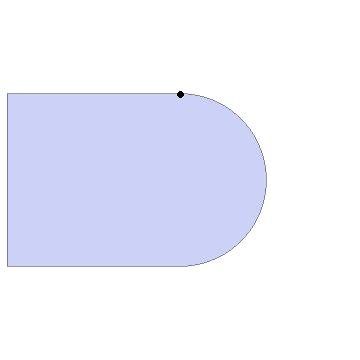
\includegraphics[width=0.5\textwidth]{nonexposed}
    \caption{The emphasized point is extreme but not exposed.}
    \label{nonexposed}
  \end{center}
\end{figure}

As already mentioned, the convex hull of a set $S \subset \R^n$ consists of convex combinations $t_1x_1+\ldots+t_kx_k$, but what is $k$? More precisely: given a set $S$, what is the smallest $k$ for which everything in $conv(S)$ is a convex combination of no more than $k$ points in $S$? It is not immediately obvious that there is such a $k$, but a theorem of Carath\'{e}odory gives the best upper bound possible given its hypotheses (see Figure \ref{Caratheodory}).

\begin{thm}(Carath\'{e}odory Convex Hull Theorem) If $S \subset \R^d$, then every element of $conv(S)$ may be expressed as a convex combination of $d+1$ or fewer elements of $S$
\label{Cara}
\end{thm}

\begin{figure}[H]
  
  \begin{center}
    
\includegraphics[width=0.5\textwidth]{Caratheodory}
    \caption{A set requiring $d+1$ summands}
    \label{Caratheodory}
  \end{center}
\end{figure}

While the bound given by Carath\'{e}odory's theorem is in this sense sharp, it is too crude for our purposes. We can say much more about convex hulls of specific sets for which we have explicit descriptions. For now we have that the pythagoras number of $\snd$ itself is no more than $\binom{n+2d-1}{2d}+1$, since $\dim \pnd$ can be shown by a ``stars and bars" counting argument to be $\binom{n+2d-1}{2d}$.

We conclude with some intuitive results which will be useful in the remaining chapters, all of which can be found in \cite{Barvinok}.

\begin{thm}
Let $S\subset \R^m$ be a convex set. If $\mathring{S} = \emptyset$, then $S$ is contained in a proper affine subspace of $\R^m$
\label{fatconvex}
\end{thm}

The next will be used to show that $\snd$ is closed. See discussion preceding \ref{SOScompact} for a definition of \emph{base}.

\begin{thm}If $C\subset \R^m$ is a cone with a compact base, then $C$ is closed.
\label{KCone}
\end{thm}

The last has several variants used extensively in functional analysis. We will use it in Chapter \ref{ch3}.

\begin{thm}(Separating Hyperplane Theorem) If $C\subset \R^m$ is a closed convex set and $x \notin C$, then there is an affine hyperplane strictly separating $x$ and $C$, that is, there exists a linear functional $\Lambda$ on $\R^m$ and a real number $r$ such that $\Lambda(y) < r$ for all $y\in C$ and $\Lambda(x) > r$.
\label{Separation}
\end{thm}

\end{section}

\begin{section}{Overview}
In the next chapter we discuss some well-known properties of the SOS cone and explain in detail its connection with the PSD cone. We survey relevant work and summarize what is currently known about pythagoras numbers. In addition, we explore noncommutative sums of `squares', and show how a theorem of Pfister fails to extend into this setting. Chapter $3$ contains the main contribution of this dissertation and deals with the more general problem of quadratic convexity. Related results from the literature are included. After reducing the cases to be considered, we prove the main result which is in turn used to derive lower bounds on pythagoras numbers. In addition, we employ the \emph{Approximate Carath\'{e}odory Theorem} in bounding the distance from the sums of $k$ squares to an arbitrary sum of squares. We conclude with Chapter $4$, where other approaches are discussed which might be used to characterize quadratic convexity.
\end{section}

\label{ch1}
\end{chapter}

				%%%%%%%%%%%%%%%
				%%%%CHAPTER 2%%%%
				%%%%%%%%%%%%%%%
								
\begin{chapter}{Sums of Squares and PSD Matrices}
We now explain the connection between PSD matrices and polynomials. We will see how the problem of computing length may be recast as a rank minimization problem. The first two sections are intended as a survey of standard techniques and well-known results. The chapter concludes with some work in the noncommutative setting.
\begin{section}{PSD, SDP and Rank}
Let us fix $p = \sum_\alpha p_\alpha x^\alpha \in \snd$. There are forms $g_1,\ldots,g_k \in \pn_d$ such that $p = g_1^2+\ldots+g_k^2$. In fact, any $g_i$ satisfying this equation must be homogeneous of degree exactly $d$ because the largest and smallest monomials occurring with nonzero coefficients in the $g_i$ will contribute nonzero terms to the sum $g_1^2+\ldots+g_k^2$. For each $i$, we may express $g_i$ as $\sum_\alpha g_{i,\alpha}x^\alpha$. Defining ${\bf g_i} = (g_{i,\alpha})_{|\alpha|=d}^T \in \R^N$ and ${\bf m} = (x^\alpha)_{|\alpha|=d}^T \in \pn_d^N$, where $N = \dim \pn_d$, we get $g_i^2 = {\bf g_i}^T {\bf m} {\bf m}^T {\bf g_i}=\trace( {\bf g_i}{\bf g_i}^T{\bf m}{\bf m}^T)$, and therefore $p = \trace({\bf m}{\bf m}^T(\sum_i{\bf g_i}{\bf g_i}^T))$. This equation is really a system of $\binom{n+2d-1}{2d}$ equations of the form $p_\alpha = \trace(A_\alpha \sum_i{\bf g_i}{\bf g_i})$, where $A_\alpha$ is the $N\times N$ matrix, indexed by multi-indices, whose entries are given by

\[(A_\alpha)_{\beta,\gamma} = 
\begin{cases}
1, & \text{if }\beta+\gamma=\alpha \\
0, & \text{otherwise }
\end{cases}
\]

With these matrices we may now define the \emph{spectrahedron associated to} $p$:
\[S(p)\equiv \{X \in S_N^+ \mid \trace(A_\alpha X) = p_\alpha \text{ for all } \alpha \text{ with } |\alpha|=2d\}.\]
In general, a \emph{spectrahedron} is a set of the form $S_m^+ \cap V$, where $V$ is an affine subspace of $\R^m$. In the case of $S(p)$, the set $V$ is the codimension $\binom{n+2d-1}{2d}$ (since the $A_\alpha$ are disjointly supported and therefore comprise a linearly independent set) affine subspace
\[\{X \in M_N(\R) \mid \trace(A_\alpha X) = p_\alpha \text{ for all } \alpha \text{ with } |\alpha|=2d\}\] 

An element of $S(p)$ is called a \emph{Gram matrix} for $p$. It was demonstrated in the discussion above that each decomposition $g_1^2+\ldots+g_k^2$ of $p$ into a sum of squares yields an element of the spectrahedron $S(p)$, namely the matrix $\sum_i{\bf g_i}{\bf g_i}$. It is also true that every element of $S(p)$ yields a decomposition of $p$ into a sum of squares. To see how, fix $X \in S(p)$ and apply \ref{PSDMat} to obtain
\[X = L^TL,\]
where $L\in M(\R)_N$. For each $1\leq i\leq N$, we now define $f_i$ to be the polynomial in the $i^{th}$ entry of $L{\bf m}$. Since $X = L^TL \in S(p)$, we get $p = \sum_if_i^2$. This yields a dramatic improvement of the bound obtained from \ref{Cara}, but the improved bound does not generally give the length of a sum of squares. In most cases, the Gram matrix is not unique. In fact, the set $S(p)$ is generally not finite. Below is an example illustrating this non-uniqueness, followed by a characterization of the cases in which $S(p)$ is a singleton. 

\begin{examp}(An explicit spectrahedron) Take $n=2$ and $d=2$. We then have $\binom{2+4-1}{4} = 5$ matrices $A_\alpha \in \s_3$ which describe $p \in \snd$: $A_{(4,0)}=\left(\begin{smallmatrix} 1 & 0 & 0 \\0 & 0 & 0\\0&0&0 \end{smallmatrix}\right)$,  $A_{(3,1)}=\left(\begin{smallmatrix} 0 & 1 & 0 \\1 & 0 & 0\\0&0&0 \end{smallmatrix}\right)$, $A_{(2,2)}=\left(\begin{smallmatrix} 0 & 0 & 1 \\0 & 1 & 0\\1&0&0 \end{smallmatrix}\right)$, $A_{(1,3)} = \left(\begin{smallmatrix} 0 & 0 & 0 \\0 & 0 & 1\\0&1&0 \end{smallmatrix}\right)$, and $A_{(0,4)}=\left(\begin{smallmatrix} 0 & 0 & 0 \\0 & 0 & 0\\0&0&1 \end{smallmatrix}\right)$. If we take $p(x,y) = x^4+x^2y^2+y^4$, then $X = \left(\begin{smallmatrix} 1 & 0 & 0 \\0 & 1 & 0\\0&0&1 \end{smallmatrix}\right)$ belongs to $S(p)$, but $S(p)$ is in fact a line segment in $\s_3^+$ which we'll now describe.

Note that $X \longmapsto (\trace(A_\alpha X))_{|\alpha|=4}$ defines a surjective linear map from $\s_3$ to $\R^5$. The kernel of this map is therefore spanned by a single matrix in $\s_3$. One such matrix is $X_0 \equiv \left(\begin{smallmatrix*} 0 & 0 & 1 \\ 0 & -2 & 0  \\ 1&0&0 \end{smallmatrix*}\right)$. We conclude that the set $S(p)$ consists of exactly the linear combinations $X+tX_0$ which are PSD. Invoking \ref{PSDMat} again we find that $X+tX_0 \succeq0$ exactly when $-1 \leq t \leq \frac{1}{2}$. It is interesting to note that each of the two boundary values yields a Gram matrix of rank $2$. It is easily verified that $2$ is the minimum value of rank on the set $S(p)$. More can be said; we will see in \ref{pythy} that $\p(\Sigma_{2,d}) = 2$ for any $d$. $\QED$
\label{example1}
\end{examp}

There is much in the preceding example to be fleshed out and generalized. Recalling the linear transformation defined above, we extend to arbitrary $n$ and $d$ in order to understand when it happens that $S(p)$ consists of the unique Gram matrix for $p$.

\begin{prop} For any $n,d \in \N$, the linear transformation $T:\s_N \to \R^M$ defined by $T(X)=(\trace(A_\alpha X))_{|\alpha|=2d}$, where $N=\binom{n+d-1}{d}$ and $M = \binom{n+2d-1}{2d}$, is surjective. The transformation $T$ is a bijection if and only if $d=1$ or $n=1$. 
\label{SN+squash}
\end{prop}

\begin{proof} There are exactly $M$ of the $A_\alpha$. Furthermore, we have $\trace(A_\alpha A_\beta) = 0$ for $\alpha \neq \beta$ from the definition. It follows that the map $T$ is surjective.

Now we assume that $d=1$ and let $n\in \N$ be arbitrary. In this case, we have $\dim \s_N = \binom{N+1}{2} = \binom{n+1}{2} = \binom{n+2-1}{2}$. By the rank-nullity theorem, $T$ must be a bijection. If we take $n=1$, then both spaces are $1-$dimensional and $T$ is a bijection.

Conversely, suppose that $d\geq 2$ and $n\geq 2$. Define an equivalence relation $\sim$ on the set of pairs of monomials in $\pn_d$ by 
\[(u,v) \sim (w,z) \iff uv=wz.\]
This partitions the set of pairs into $M$ disjoint equivalence classes (this will be justified rigorously in the next section), but some of these classes are not singletons. Consider for instance the monomial $x_1^dx_2^d=(x_1^{d-1}x_2)(x_1x_2^{d-1})$, and note that because $d-1>0$, these are really two distinct decompositions.
\end{proof}

It follows from this proposition and the convexity of $S(p)$ that it is finite only in the simple cases $d=1$ and $n=1$. And we obtain another description of this set in terms of the kernel of the map $T$ above.

\begin{prop} If $p\in \snd$ and $T$ is as above, then for any $X_p$ satisfying $T(X_p) = (p_\alpha)_{|\alpha|=2d}$ we have
\[S(p) = \{ X \in \s_N^+ \mid X-X_p \in \ker T\}\]
\label{kernelSDP}
\end{prop}

We also saw in \ref{example1} that the length of our particular $p$ was obtained on the boundary of $S(p)$, at Gram matrices of smallest possible rank. This holds in general.

\begin{prop} If $p \in \snd$, then $\ell(p) = \min \{\rank(X)\mid X \in S(p)\}$.
\label{RankLength}
\end{prop}
\begin{proof}
Let $X \in S(p)$. Since $X$ is symmetric, the spectral theorem yields a decomposition $U^TDU=X$, where $U$ is orthogonal and $D$ diagonal, with the eigenvalues $\lambda_i$ of $X$ along the diagonal. If we denote by $U_i$ the $i^{th}$ row of $U$, then we have
\[p =\trace({\bf m}{\bf m}^TX)= \trace({\bf m}^TU^TDU{\bf m})=\sum_i \lambda_i (U_i{\bf m})^2\]
where ${\bf m}$ is the monomial vector introduced in the discussion preceding \ref{example1}. The rank of $X$ is exactly the number of nonzero eigenvalues $\lambda_i$, which in turn is the number of squares in the sum.
\end{proof}

This observation does not make our task easier. In fact, it is shown in \cite{BoydVand} that rank minimization is NP-Hard. Heuristics exist for rank minimization which succeed in many cases, as demonstrated in \cite{FAZ} and \cite{CandTao}. They succeed sometimes. The work of Recht, Fazel and others (\cite{FAZ}) does not help us here because we are not concerned with restricted isometries. But \ref{example1} does in fact give an example where trace minimization produces solutions of minimum rank. 

 We just saw a rudimentary instance of semidefinite programming which could be done by hand. Formally, a \emph{semidefinite program} (SDP) is an optimization problem of the form

\begin{equation*}
\begin{aligned}
& \text{minimize}
& & \trace(CX) \\
& \text{subject to}
& & \trace(A_iX) = b_i\\
&&& X \succeq 0,
\end{aligned}
\end{equation*}
where $C$ and $A_i$ are square matrices and $b_i$ are real numbers. The formulation above is called the \emph{primal} SDP. The \emph{dual} to this problem is:

\begin{equation*}
\begin{aligned}
& \text{maximize}
& & a^Ty \\
& \text{subject to}
& & \sum_i y_iA_i +S = C\\
&&& S \succeq 0.
\end{aligned}
\end{equation*}

In both of these optimization problems, the feasible region is a spectrahedron (or at least isometrically isomorphic to one). Because we can lift any functional to a functional on a higher dimensional space, the feasible regions of SDPs are exactly linear images of spectrahedra. In the next section, we show that the set $\snd$ is exactly such an image. In fact, certain other sets of polynomials related to $\snd$ can be realized as such, and therefore optimization of linear functionals over those sets can be done via SDP.

The \emph{quadratic module} generated by $g_1,\ldots,g_m \in \pn$, denoted $Q(g_1,\ldots,g_m)$, is the set of all sums of the form $\sum_{i=0}^m g_i\sigma_i$, where $g_0 \equiv 1$ and each $\sigma_i$ is a sum of squares. The $k^{th}$ \emph{truncated quadratic module} is the set 
\[Q_k(g_1,\ldots,g_m) = \Big\{\sum_{i=0}^m g_i\sigma_i \mid \sigma_i \text{ is SOS and } \deg(g_i\sigma_i) \leq 2k \text{ for every } i\Big\}.\]
A truncated qudratic module is also a projected spectrahedron, since it is an image under a linear transformation of another projected spectrahedron, namely $\snd$ (recall \ref{SOSspect}). Under additional assumptions on the polynomials $g_1,\ldots,g_m$, it has been shown (in \cite{Lass1}, for instance) that the optima \[\lambda_k = \max \lambda \text{ s.t } f-\lambda \in Q_k(g_1,\ldots,g_m)\] converge to the minimum of the polynomial $f$ on the set \[\{x \mid g_i(x) \geq 0 \text{ for all }i\}.\]

\end{section}

\begin{section}{Properties of the SOS Cone}
We present some important properties of the SOS cone and justify the claims made in the proof of \ref{SN+squash}. In some of the results below, polynomials are identified with their coefficient vectors in $\R^M$; the monomials are identified with the standard basis vectors for $\R^M$, and we use the euclidean topology.

\begin{prop} The set $\snd$ is a convex cone of full dimension in $\pn_{2d}$.
\label{SOSfullD}
\end{prop}
The idea of the proof is to show that $\snd$ is not contained in a proper subspace of $\pnd$. Since it is convex, this implies that it has nonempty interior.
\begin{proof} The convexity of $\snd$ is trivial: if $g_1^2+\ldots+g_k^2,$ $f_1^2+\ldots+f_\ell^2 \in \snd$, and $t \in [0,1]$, then $t(g_1^2+\ldots+g_k^2)+(1-t)(f_1^2+\ldots+f_\ell^2)=$
\[(\sqrt{t}g_1)^2+\ldots+(\sqrt{t}g_k)^2+(\sqrt{1-t}f_1)^2+\ldots+(\sqrt{1-t}f_\ell)^2 \in \snd.\]
It remains to show that the set of squares of polynomials in $\pn_d$ is contained in no proper affine subspace of $\R^M$. Together with \ref{fatconvex}, this will prove the claim. We prove that the squares span $\R^M$ (rather, their coefficient vectors do).

Let $x^\alpha \in \pnd$. Now construct $\beta$ and $\gamma$ as follows: if $\alpha_k$ is even, then we set $\beta_k = \gamma_k = \frac{1}{2}\alpha_k$. If $\alpha_k$ is odd, then we set one of $\beta_k$ and $\gamma_k$ equal to $\alpha_k-1$ and the other to $\alpha_k+1$. Since $2d$ is even, \emph{the number of odd $\alpha_ks$ must be even}. We can therefore assign half of the decremented values ($\alpha_k-1$) and half of the incremented values ($\alpha_k+1$) to each of $\beta$ and $\gamma$ to obtain $x^\beta$ and $x^\gamma$ in $\pn_d$ satisfying $x^\alpha = x^\beta x^\gamma$. Finally, we compute
\[x^\alpha = \frac{1}{4}(x^\beta +x^\gamma)^2 - \frac{1}{4}(x^\beta-x^\gamma)^2,\]
which completes the proof.
\end{proof}

The next proposition will be used in Chapter $4$ to give an alternative formulation of the problem.

\begin{prop} The set $\snd$ is a projected spectrahedron.
\label{SOSspect}
\end{prop}
\begin{proof} Recall the map from \ref{SN+squash}. In the remarks preceding \ref{example1}, we proved that $\snd = T(\s_N^+)$.
\end{proof}

Before stating \ref{SOScompact}, we need a new term. A convex subset $K$ of a  convex cone $C$ is called a \emph{base} if for every nonzero $x \in C$ there is exactly one positive $t \in \R$ for which $tx \in K$. 

\begin{prop}The set $\snd$ has a compact base.
\label{SOScompact}
\end{prop}

\begin{proof}Define $K = \{ p \in \snd \mid \int_{[0,1]^n}p = 1\}$, where $\int_{[0,1]^n}$ is the integral with respect to Lebesgue measure over the unit cube in $\R^n$. We show that $K$ is a compact base for $\snd$. If $p \in \snd$ is nonzero, then $\int_{[0,1]^n}p > 0$. This follows from the fact that a nonzero polynomial is a continuous function nonzero almost everywhere; since $p$ is positive at some point, $p$ is positive on an open subset of $[0,1]^n$. Defining $t$ by $t\int_{[0,1]^n}p = 1$, we get $tp \in K$. Uniqueness of $t$ is obvious.

It remains to show that $K$ is compact and convex. Convexity of $K$ follows easily from linearity of $\int_{[0,1]^n}$ as a linear functional. To prove that $K$ is compact, we realize $K$ as the image of a compact set under a continuous map. Define 
\[K' = \big\{p \in \pn_d \mid \|p\|_2 = 1\big\}^N\times \Delta^{N-1},\]
and $f: (\pn_d)^N\times \Delta^{N-1} \to \pnd$ by $f(p_1,\ldots,p_N,t_1,\ldots,t_N) = \sum_j t_jp_j^2$, where $\Delta^{N-1}$ is the standard simplex in $\R^N$, and $\|\cdot\|_2$ is the $L^2$ norm. The set $K$ is equal to $f(K')$ by construction, and is therefore compact.
\end{proof}
A cone with a compact base is called \emph{proper}. The terms is used in other senses, but this will do for all cases handled here. In Chapter $3$ we will realize \ref{SOScompact} as a special case of a general theorem about quadratic maps; we could find a compact base by constructing a positive definite linear combination of the $A_\alpha$.

Here is one last property of the cone $\snd$ itself which we will meet again, but in more generality, in the next chapter.
\begin{cor} The set $\snd$ is closed.
\label{SOSclosed}
\end{cor}
\begin{proof} This follows from \ref{SOScompact} and \ref{KCone}.
\end{proof}

\begin{examp}
Here is a concrete example of a compact base for $\snd$. Taking $n=d=2$, with notation as in \ref{example1}, we note that the linear combination
\[B\equiv A_{(4,0)}+\tfrac{1}{2}A_{(3,1)}+\tfrac{1}{3}A_{(2,2)}+\tfrac{1}{4}A_{(1,3)}+\tfrac{1}{5}A_{(0,4)}\]
is positive definite (since $B$ is a truncated Hankel matrix of Lebesgue measure on the unit interval). Define 
\[C = \{ X \in \s_3^+ \mid \trace(XB) = 1\},\]
and $K=T(C)$. Since $C$ is a compact (by positive definiteness of $B$) convex set and $T$ is linear, $K$ must be a compact convex set. Suppose that $p \in \snd$ is not zero. Then there exists $X_p \in \s_3^+$ such that $T(X_p) = p$. Since $X_p \succeq 0$ and $B \succ 0$, we have $\trace(X_pB) >0)$. Thus, $\tfrac{1}{\trace(X_pB)}p \in K$. To see that this is the unique positive multiple of $p$ belonging to $K$, note that whenever $X \in S(p)$ we must have $\trace(A_\alpha(X-X_p))=0$ for all $\alpha$, so that $\trace(B(X-X_p)) = 0$. That is, the functional $\trace(B\cdot)$ is constant on $S(p)$. $\QED$
\label{example2}
\end{examp}

Finally, we mention the \emph{Motzkin form}, a nonnegative polynomial which is not SOS.

\begin{examp}Define $M(x,y,z) = x^2y^4+x^4y^2+z^6-3x^2y^2z^2$. That $M$ is nonnegative follows from the arithmetic-geometric mean inequality. Using \ref{NewtLatt}, it can be shown that $M$ is not SOS. To see how, let us examine the \emph{Newton polytope} C(M) of $M$. 
\[C(M) = \conv \Big \{\Big(\begin{smallmatrix}2\\4\\0\end{smallmatrix}\Big),\Big(\begin{smallmatrix}4\\2\\0\end{smallmatrix}\Big),\Big(\begin{smallmatrix}0\\0\\6\end{smallmatrix}\Big),\Big(\begin{smallmatrix}2\\2\\2\end{smallmatrix}\Big)\Big\},\]so that if $M=g_1^2+\ldots+g_k^2$ we must have for each $j$ \[C(g_j) \subset \conv \Big \{\Big(\begin{smallmatrix}1\\2\\0\end{smallmatrix}\Big),\Big(\begin{smallmatrix}2\\1\\0\end{smallmatrix}\Big),\Big(\begin{smallmatrix}0\\0\\3\end{smallmatrix}\Big)\Big\}. \]
Since $\Big(\begin{smallmatrix}1\\2\\0\end{smallmatrix}\Big),\Big(\begin{smallmatrix}2\\1\\0\end{smallmatrix}\Big),\Big(\begin{smallmatrix}1\\1\\1\end{smallmatrix}\Big),$ and $\Big(\begin{smallmatrix}0\\0\\3\end{smallmatrix}\Big)$ are the only integer points in $\tfrac{1}{2}C(M)$ (see Figure \ref{Motzkin}), the assumption that $M=g_1^2+\ldots+g_k^2$ implies that $x^2y^2z^2$ must appear with a positive coefficient in $M$. Since this is not the case, we conclude that $M$ is not a sum of squares.
$\QED$
\end{examp}

\begin{figure}[H]
  
  \begin{center}
    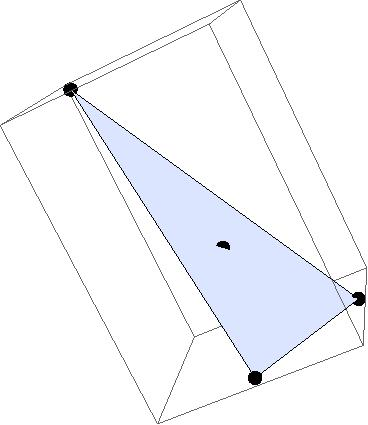
\includegraphics[width=0.5\textwidth]{Motzkin}
    \caption{$\tfrac{1}{2}C(M)$. Emphasized points are integer lattice points.}
    \label{Motzkin}
  \end{center}
\end{figure}

Combining the example above with \ref{SOSclosed}, we conclude that for some values of $n$ and $d$ the cone of nonnegative polynomials in $\pnd$ contains an open ball disjoint from $\snd$. It is natural to ask how much ``smaller" $\snd$ is. One way to compare the two cones is to compare corresponding compact bases - nonnegative polynomials integrating to $1$ on the unit cube also comprise a compact base for the nonnegative cone. In \cite{blek2}, Blekherman showed that if degree is fixed and the number of indeterminates allowed to grow, then the base of SOS shrinks to an arbitrarily small proportion of the base of the nonnegative forms. 

\label{SOSprops}
\end{section}





\begin{section}{Bounds on $\p(\pnd)$}
It is known that $\p(\Sigma_{2,d})=2$, that $\p(\Sigma_{n,1}) = n$ and that $\p(\Sigma_{3,2})=3$. For arbitrary $n$ and $d$ there are explicit upper and lower bounds on $\p(\snd)$ which generally do not coincide. As we saw in Chapter $2$, it holds for all $n$ and $d$ that $\p(\pnd) \leq \dim \pn_d$. Better bounds are given in \cite{RezChoiLam}, where the authors use the method of \emph{cages} - a generalization of the Newton polytope.

\begin{defn}For a form $ p= \sum_\alpha p_\alpha x^\alpha \in \pnd$, we define the \emph{Newton polytope} of $p$, denoted $C(p)$, to be the convex hull of the set $\{\alpha \mid p_\alpha \neq 0\}$ (recall that the $\alpha$ belong to $\R^n$).
\end{defn}

A property of the Newton polytope used in \cite{RezChoiLam} (and proved in \cite{RezNewt}) to obtain bounds on the the pythagoras numbers of certain subsets of $\pnd$ also provides an easy way to show that the Motzkin form is not SOS. While eminently plausible, this result is not trivial. In particular, it is much stronger than the observation that $\alpha = \tfrac{1}{2}(2\alpha)$.

\begin{thm}If $f =g_1^2+\ldots+g_k^2$, then $C(g_i) \subset \tfrac{1}{2}C(f)$ for each $i = 1,\ldots,k$.
 \label{NewtLatt}
 \end{thm}

Let $a$ denote the dimension of $\pnd$, and $e$ that of $\pn_d$. Here are the bounds given in \cite{RezChoiLam}:

\begin{thm} 
\[\frac{2e+1-\sqrt{(2e+1)^2-8a}}{2} \leq \p(\pnd) \leq \frac{\sqrt{1+8a}-1}{2}\]
\end{thm}
The lower bound is sharp in many cases, but the upper bound agrees in only a few cases. The upper bound can be obtained from a bound on rank in spectrahedra presented in \cite{Barvinok}. We now turn to sums of squares of \emph{noncommutative} polynomials to see how their lengths behave differently.
\label{pythy}
\end{section}


\begin{section}{The NC Setting and Pfister's Theorem}
In this section we present related work on sums of squares of noncommutative polynomials originally published in \cite{billbook}, reused here with kind permission of Springer Science+Business Media. First, we must define new objects and mention some noncommutative results.  We work in the real free $\ast$-algebra $\R\langle X, X^* \rangle$ generated by the $n$ noncommuting (NC) variables $X_1, \ldots, X_n$ and their \emph{adjoints} $X_j^*$.  We can think of these variables as linear operators, and the $\ast$ function on $\R\langle X, X^* \rangle$ as the adjoint operation.  In particular, $\ast$ respects addition and multiplication by scalars and is defined on monomials by $(X_{j_1} \cdots X_{j_k}) ^*= X_{j_k}^* \cdots X_{j_1}^*$ and $(X_j^*)^*=X_j$.  We use multi-indices $\alpha$, tuples of non-negative integers from $0$ to $2n$, to index monomials: $X^\alpha \equiv X_{\alpha_1}X_{\alpha_2} \cdots X_{\alpha_k}$. The word $X^\emptyset$ is simply the empty word, denoted by $1$.  For $0<j\leq n$, we define $X_{j+n} \equiv X_j^*$.  Conjugation and concatenation of multi-indices $\alpha$ and $\beta$ is defined by the equations $X^{\alpha^*}=(X^\alpha)^*$ and $X^{\alpha \circ \beta}  = X^{\alpha} X^{\beta}$.

Evaluation of $p \in \R\langle X, X^* \rangle$ at a tuple $(M_1, \ldots, M_n)$ of square matrices of common size is defined by the substitution of $M_j$ for $X_j$ and $M_j^T$ for $X_j^*$.

We say that $p \in \R\langle X, X^* \rangle$ is symmetric when $p^*=p$.  Such a polynomial $p$ is said to be \emph{matrix positive} if the matrix $p(M)$ is positive semidefinite (or \emph{PSD}) for every tuple $M$ of square matrices.  It was shown by Helton in \cite{HE} that every matrix positive polynomial is a sum of squares.  The minimal number of squares required to express a matrix positive polynomial as a sum of squares is not known in general, although upper bounds are easy to obtain.  

Optimization in certain quantum physics problems is done over feasible regions of operators on Hilbert spaces, and so NC variables are useful there. Several examples and a general framework for such problems are presented in \cite{PIR}, where the semidefinite programming relaxations of Lasserre are extended to the NC setting. Motivation for the study of NC polynomials from control theory is discussed in \cite{HE2}.

To any symmetric polynomial $p \in \R\langle X, X^* \rangle$ we can associate a real, symmetric matrix $M$ with the property

\[ V^*MV=p\]

where $V^*=(X^{\alpha^*})_{|\alpha|\leq d}$, and $V$ is the column vector $(X^{\alpha})_{|\alpha|\leq d}^T$ (with the monomials in graded lexicographical order). The matrix $M$ is not unique, in fact the set of all such matrices (for a fixed p) forms an affine space which we will denote $\mathcal M_p$.

By the rank of $p$, we mean the minimum of $\text{rank}(M)$ over all $M\in \mathcal {M}_p$.  For a positive polynomial, this minimum is to be taken over only the PSD matrices.  The following lemma helps us obtain a lower bound on rank.

\begin{lem}
If $A$ is a symmetric matrix satisfying $V^*AV=0$, then the $(2n)^d\times (2n)^d$ lower right submatrix of $A$ is the zero matrix.
\end{lem}

\begin{proof} Let $B$ denote the block in question, and $\hat V$ the tautological vector of just the monomials of degree $d$. Then $V^*AV=0$ implies that $\hat V^* B \hat V=0$ as well since the product $\hat V^* B \hat V$ yields exactly the degree $2d$ terms of the polynomial $V^*AV$. But the entries of $B$ are exactly the coefficients of the distinct monomials in $\hat V^*B\hat V$, hence $B$ is the zero matrix.\end{proof}

The lemma above shows that there is no freedom in choosing the block corresponding to the degree $2d$ terms of the polynomial. Since the rank of this block gives a lower bound on the rank of the whole matrix, taking the block to be the the $(2n)^d\times (2n)^d$ identity yields a polynomial with rank at least $(2n)^d$.

As already mentioned, the cone of positive polynomials properly contains the SOS cone (recall the Motzkin form). In contrast, the NC setting offers the nice result, proved by Helton in \cite{HE}, that any positive polynomial is a sum of squares.  Here, a square takes the form $f^*f$, so that a sum of squares is positive in the sense defined above. Just as in the commutative case, we have a simple relationship between SOS and the PSD cones.

\begin{lem}
A polynomial $p$ is matrix positive exactly when it can be expressed $p=V^*MV$, with $M$ a PSD matrix.  
\end{lem}

The proof is straightforward.  It follows that the \emph{length} of $p$ is 
\[\min \hspace{.5cm}  \text{rank  }X\]
\[\hspace{1cm} \text{s.t.   } V^*XV=p,\]
\[\hspace{2cm} X \succeq 0,\] 
just as in the commutative setting.


As a simple example of this problem consider the polynomial \[P=1+X^*X+XX^*,\] clearly a sum of squares. The polynomial $P$ is a sum of $3$ squares, but can be expressed as a sum of $2$ squares (and no fewer).  To see why we parametrize the affine space $\mathcal M_P$ by the single parameter $t \in \R$.  As usual  $V=(1,X,X^*)^T$, and so $P=V^*V=X^*X+XX^*+1$. Defining 
\[M=\left(\begin{smallmatrix} 
 0 & 1 & -1\\
 1 & 0 &0\\
  -1 & 0& 0
\end{smallmatrix}\right),\]

we get $\mathcal M_P= \{I+tM \mid t\in \R\}$, and find the minimal SOS representation $$P=\Big(X+\frac{\sqrt{2}}{2}\Big)^*\Big(X+\frac{\sqrt{2}}{2}\Big) +\Big(X^*-\frac{\sqrt{2}}{2}\Big)^*\Big(X^*-\frac{\sqrt{2}}{2}\Big) $$
on the boundary of the region where $I+tM \succ 0$. Note that in this example trace is constant on $\mathcal M_P \cap PSD$, and that the given solution is obtained by maximizing $t$ over $\{t\mid I+tM \succeq 0\}$.

Pfister's Theorem (proved in \cite{PFIST}) gives a bound on the number of rational functions in the SOS representation of a PSD polynomial. The bound is remarkable because it does not depend on the degree of the polynomial in question. D'Angelo and Lebl proved in \cite{DAN} that this result fails for Hermitian polynomials.  We'll show that it fails for noncommutative polynomials. The first theorem below is needed for the second. It is easy to check that the polynomial $S$ below has length $(2n)^d$, but more is true. 
\begin{thm}
Suppose that $q \in \R\langle X, X^*\rangle$ and define $S=\sum_{|\alpha|=d} X^{\alpha^*}X^\alpha$. Then $p=q^*Sq$ has length at least $(2n)^d$.  Here, $(2n)^d$ is the dimension of $span\{X^\alpha\}_{|\alpha|=d}$.
\label{threepointone}
\end{thm}

\begin{proof} Since $p$ is matrix positive, it is a sum of squares, and so we may write $p = V^*MV$, appending $V$ with the necessary monomials.  Let $q$ be such that $q^*Sq=p$, and write $q= \sum_\alpha q_\alpha X^\alpha$.  Let $\hat \alpha$ be maximal, with respect to lexicographical ordering, among all $\alpha$ such that $q_\alpha \neq 0$.

We have $V^*MV=p=q^*Sq=q^*( \sum_{|\alpha|=d} X^{\alpha^*}X^\alpha)q=\sum_{|\alpha|=d} (X^{\alpha}q)^*(X^\alpha q)$. For each $\alpha$, write $X^\alpha q= Q_\alpha V$, where $Q_\alpha$ is the row vector of the coefficients of $X^\alpha q$.  Forming the matrix $Q$ whose rows are the $Q_\alpha$ we get $V^*MV=p=V^*Q^*QV$, hence $V^*(M-Q^*Q)V=0$.  

The polynomials $X^\alpha q$ form a linearly independent set, and in fact have the distinct leading terms $q_{\hat \alpha}X^{\alpha \circ \hat \alpha}$.  It follows that the last $(2n)^{d+deg(q)}$ columns of $Q$ form a block of rank at least $(2n)^d$.  Writing $Q$ in block form $Q=\begin{bmatrix}A&B\end{bmatrix}$ where $B$ is a $(2n)^d\times (2n)^{d+deg(q)}$ matrix, we compute

\[p=V^*Q^TQV=V^*\begin{bmatrix} A^T \\ B^T \end{bmatrix} \begin{bmatrix}A&B\end{bmatrix}V=V^*\begin{bmatrix}A^TA & A^TB\\ B^TA & B^TB\end{bmatrix}V.\]


The $V$ above includes all monomials up to degree $(2n)^{d+deg(q)}$.  Since $V^*(M-Q^*Q)V=0$, we know from the lemma that $M$ cannot differ from $Q^*Q$ in its $(2n)^{d+deg(q)}\times (2n)^{d+deg(q)}$ lower right block; this block equals $B^TB$.  Therefore $M$, an arbitrary matrix representation for $p$, has rank at least $(2n)^d$.\end{proof}

Alternatively, one might ask whether a Pfister's Theorem holds for products of the usual form. Consider what it would take for $q^*qS$ to be a SOS.  Because $q^*q$ is symmetric, we note that since SOS are symmetric we must have $q^*qS=(q^*qS)^*=Sq^*q$, so that $q^*q$ and $S$ commute.  Since we evaluate these polynomials on tuples of matrices, it is tempting to treat them as symmetric matrices.  In particular, one might guess that if two of them commute, then they are both polynomials in a third polynomial. This happens to be true, and it follows from the following more general theorem from combinatorics.

\begin{thm}
(Bergman's Centralizer Theorem) Let $K$ be a field, and $K\langle X\rangle$ the ring of polynomials over $K$ in noncommuting variables $X_1,\ldots,X_n$.  Then the centralizer of a nonscalar element in $K\langle X\rangle$ is isomorphic to $K[t]$ for a single variable $t$.
\label{Bergman}
\end{thm}
The proof is a bit lengthy and can be found in \cite{LO}.  It uses the fact that such a centralizer is integrally closed in its field of fractions together with an easier result in the formal series setting.

\begin{thm}(Cohn's Centralizer Theorem) Let $K$ be a field and $K\langle \langle X \rangle \rangle$ the ring for formal power series over $K$ in noncommuting variables $X_1, \ldots,X_n$. Then the centralizer of a nonscalar element in $K\langle \langle X \rangle \rangle$ is isomorphic to $K[t]$ for a single variable $t$.

\end{thm}

These theorems apply despite the superficial difference that we are working with indeterminates $X_1,\ldots,X_n,X_1^*, \ldots,X_n^*$ for which $(X_i^*)^*=X_i$; there are no \emph{polynomial} relations among them, and so we can regard them as $2n$ noncommuting variables $Y_1, \ldots,Y_{2n}$. Armed with \ref{Bergman}, we are ready to give the counterexample. 

\begin{thm}

If $p \in \R\langle X, X^*\rangle$, a matrix positive polynomial, is of the form $q^*qS$ with $S=\sum_{|\alpha|=d} X^{\alpha^*}X^\alpha$, then $l(p) \geq (2n)^d$. 
\end{thm}
\proof We will use the previous \ref{threepointone} together with Bergman's Centralizer Theorem.  The main difficulty lies in showing that under the hypotheses, $q^*q$ is actually a polynomial in $S$.

Invoking the centralizer theorem we write $q^*q=f(h(X,X^*))$ and $S=g(h(X,X^*))$ for $h(X,X^*) \in \R\langle X,X^*\rangle$ and $f(t),g(t) \in \R[t]$. It follows from the equation $S=g(h(X,X^*))$ that $g$ must have degree $1$.  To see why, write 

\[h(X,X^*)=c_1X^{\alpha_1}+\ldots+c_lX^{\alpha_l}+(\text{\emph{lower degree terms}}), \hspace{1cm}g(t)=a_kt^k+\ldots+a_0\]

with $c_j,a_i \in \R$. We note that each term $X^{\alpha_{j_1}}\cdots X^{\alpha_{j_k}}$ is symmetric since it must be one of the monomials $X^{\alpha^*}X^\alpha$ in $S$. Supposing $k>1$, we have always that $\alpha_{j_1}=\alpha_{j_k}^*$. This implies that there is just one $\alpha_j$, which is certainly not the case.  Therefore $\text{deg}(g)=1$ and we write $g(t)=at+b$ so that $S=g(h(X,X^*))=ah(X,X^*)+b$ or $h(X,X^*)=1\slash a(S-b)$.

Now we have $q^*q=f(1\slash a (S-b))=r(S)$ for some polynomial $r(t)\in \R[t]$.  Since $r(S)$ has length equal to 1(it can be expressed as a single noncommutative square), it follows that $r(t)$ is of even degree.  If not, write $r(t)=r_{2k+1}t^{2k+1}+\ldots +r_0$ with $r_{2k+1}\neq0$. Then $r(S)=r_{2k+1}S^{2k+1}+(\text{\emph{lower degree terms}})$ and we have by \ref{threepointone} that $S^{2k+1}=S^kSS^k$ and therefore $r(S)$ itself has length at least $(2n)^d>1$, a contradiction.  Finally, $tr(t)$ has odd degree and therefore another application of \ref{threepointone} lets us conclude that $p=Sr(S)$ has length at least $(2n)^d$.\endproof 

\label{NCPfister}

\end{section}
\label{ch2}
\end{chapter}


%%%%%%%%%%%%%%%%
%%%CHAPTER 3%%%%%%
%%%%%%%%%%%%%%%%

\begin{chapter}{Quadratic Convexity}
\begin{section}{The Basic Problem}
Given a tuple $A=(A_1,\ldots,A_M)$ of matrices $A_j \in \s_N$, we are interested in determining whether the sets $A(\R^N) \equiv \{(x^TA_1x,\ldots,x^TA_Mx) \mid x\in \R^N\}$ and 
$A(S^{N-1}) \equiv \{(x^TA_1x,\ldots,x^TA_Mx) \mid x\in S^{N-1}\}$ are convex. We will show how the problems are related to each other, and we will derive necessary conditions for convexity of $A(\R^N)$ and $A(S^{N-1})$. First, we mention some related work.

In Chapter \ref{ch1} we mentioned \emph{joint numerical range}, defined for tuple $A=(A_1,\ldots,A_M)$ of $N\times N$ Hermitian matrices to be the set
\[w(A) = \{(z^*A_1z,\ldots,z^*A_Mz)^T\mid z\in \C^N \text{ and } \|z\|=1\},\]
where $z^*\equiv (\bar z_1,\ldots,\bar z_N)$ and $\|z\|^2 \equiv \sum_j \bar z_j z_j$ for any vector $z \in \C^N$. It was shown in \cite{Gut1} that $w(A)$ is convex under certain conditions on the lead eigenvalue of combinations $\sum_j \eta_j A$ with $\|\eta\| =1$, though the converse is false (as is demonstrated in \cite{Gut1}). A simpler sufficient condition is the simultaneous diagonalizability of the $A_j$ or, equivalently, the condition that all pairs commute. This appears in \cite{Barvinok} as an exercise, and in \cite{BindingLi} alongside results relating boundary points of $w(A)$ to the joint spectrum of $A$. 

But the joint numerical range is just the image of a sphere under a special kind of quadratic map. Indeed, the map $z \mapsto (z^* A_1 z, \ldots, z^* A_M z)$
can be regarded as a quadratic map from $\R^{2n}$ to $\R^{2M}$ by identifying $\C$ with $\R^2$. Under this identification, the set $\{z : \|z\| = 1\}$ is of course identified with $S^{2N-1} \subset \R^{2N}$.
\end{section}

\begin{section}{Quadratic Maps and a Necessary Condition}
We begin with a theorem which enables us to modify a quadratic map $A$ in such a way that convexity (or lack thereof) is preserved, but the hypotheses of our main theorem are satisfied. A \emph{quadratic map} from $\R^N$ to $\R^M$ is a function given by $x \mapsto (x^TA_1x,\ldots,x^TA_Mx)$, where the $A_j$, for all $j = 1,\ldots,M$, are symmetric matrices. If $A=(A_1,\ldots,A_M)$ is a tuple of symmetric matrices, we will write $A(x)$ for the vector $(x^TA_1x,\ldots,x^TA_Mx)^T\in \R^M$, and abuse notation by calling $A$ itself a quadratic map.

\begin{thm} Suppose $A : \R^N \to \R^M$ is a quadratic map. Then there is a linear operator $T:\R^M\to \R^k$ satisfying
\begin{list}{\roman{qcounter})}{\usecounter{qcounter}}
\item $(T \circ A)(\R^N)$ is contained in no proper subspace of $\mathbb{R}^k$, and
\item $(T \circ A)(\R^N)$ is convex if and only if $A(\R^N)$ is convex.
\end{list}
\label{SquashFullD}
\end{thm}
\begin{proof}Take $U$ to be the orthogonal projection onto the span of $A(\R^N)$, and $V$ to be a linear isometry from that span to $\R^k$, where $k = \dim \operatorname{span}A(\R^N)$. Set $T = VU$. Then property \emph{i)} is immediate. For property \emph{ii)}, note that $A(\R^N) = U(A(\R^N))\simeq T(A(\R^N))$
\end{proof}

While the above observation is fairly straightforward, it is slightly less obvious that the analogous thing can be done in the case of $A(S^{N-1})$.

\begin{thm}Suppose $A : \R^N \to \R^M$ is a quadratic map. Then there is a linear operator $T:\R^M\to \R^k$ satisfying
\begin{list}{\roman{qcounter})}{\usecounter{qcounter}}
\item $(T \circ A)(S^{N-1})$ is contained in no proper affine subspace of $\mathbb{R}^k$, and
\item $(T \circ A)(S^{N-1})$ is convex if and only if $A(S^{N-1})$ is convex.
\end{list}
\label{SquashCompact}
\end{thm}

\begin{proof} Define the linear transformation $L :\s_N \to \R^M$ by $L(X)_i = \trace(A_iX)$ for all $i = 1,\ldots,M$, and let $W$ be the subspace $L(\kernel(\trace))$ of $\R^M$. Now take $U$ to be the orthogonal projection onto $W$ and suppose that $F$ is an affine subspace of $W$ containing $U(A(S^{N-1}))$. Then $F$ also contains the affine hull of $U(A(S^{N-1}))$, which is exactly the set $UL(\{X \in \s_N \mid \trace(X) = 1\})=W \simeq \R^{\dim W}$. Once again, take $T$ to be the composition of $U$ with a linear isometry from $W$ to $\R^{\dim W}$.

To establish property \emph{ii)}, we simply show that the two sets $U(A(S^{N-1}))$ and $A(S^{N-1})$ are translates of each other. Fix $p \in S^{N-1}$ and note that

\begin{align*}
-A(p)+A(S^{N-1}) &=L(-pp^t)+L(\{xx^t: x \in S^{n-1}\})=L(\{xx^t-pp^t: x \in S^{n-1}\})\\
&= UL(\{xx^t-pp^t: x \in S^{n-1}\} =-U(A(p))+U(A(S^{n-1})).
\end{align*}

\end{proof}

We reiterate that the above theorems are relevant because they enable to modify an arbitrary quadratic map so that the hypotheses of our two main results are satisfied. While the the convexity of $A(S^{N-1})$ and $A(\R^N)$ are not equivalent, there is an implication in one direction.

\begin{prop}Suppose that $A : \R^N \to \R^M$ is a quadratic map. Let $B$ denote the unit ball $\{x \in \R^N \mid \|x\| \leq1\}$ in $\R^N$. Then $A(\R^N)$ is convex whenever $A(B)$ is convex, and $A(B)$ is convex whenever $A(S^{N-1})$ is convex.
\label{WaferBallCone}
\end{prop}

\begin{proof}Let $A$ be as above and suppose that $A(B)$ is convex. Fix $x_1,x_2 \in \R^N$, and $t \in [0,1]$ and assume $0\neq \|x_1\| \geq \|x_2\|$. Then $(1\slash \|x_1\|)x_j \in B$ for $j=1,2$, and by convexity of $A(B)$ there exists $x \in B$ such that \[A(x) = tA\Big(\frac{1}{\|x_1\|}x_1 \Big)+(1-t)A\Big(\frac{1}{\|x_1\|}x_2 \Big).\] Multiplying this equation by $\|x_1\|^2$ completes the proof of the first implication (since $A(cv)=c^2A(v)$ for all $c \in \R$ and all $v \in \R^N$).

Now assume that $A(S^{N-1})$ is convex, and fix $x_1,x_2 \in B$, and $t \in [0,1]$. Assume that both $x_j$ are nonzero (the alternative being a trivial case). There exists $x \in S^{N-1}$ such that \[A(x) = \frac{t\|x_1\|^2}{t\|x_1\|^2+(1-t)\|x_2\|^2}A\Big(\frac{1}{\|x_1\|}x_1\Big)+\frac{(1-t)\|x_2\|^2}{t\|x_1\|^2+(1-t)\|x_2\|^2}A\Big(\frac{1}{\|x_2\|}x_2\Big).\] Multplying by $t\|x_1\|^2+(1-t)\|x_2\|^2$ we find \[A\Big(\sqrt{t\|x_1\|^2+(1-t)\|x_2\|^2}x\Big) = tA(x_1)+(1-t)A(x_2).\] Since $x \in S^{N-1}$ and $\sqrt{t\|x_1\|^2+(1-t)\|x_2\|^2} \leq 1$, we have shown that $A(B)$ is convex.
\end{proof}

Now we give two theorems regarding quadratic maps whose hypotheses generalize the properties of quadratic maps arising from parametrization of sums in $\snd$. The first reduces a broad class of quadratic maps to positive definite quadratic maps, and yields a corollary which can be seen as a partial converse to \ref{WaferBallCone}. This can be combined with the  \emph{Approximate Carath\'{e}odory Theorem} to bound the distance of elements in the convex hull to the original image. The second gives a simple necessary condition for quadratic convexity which yields, through recent results in convex algebraic geometry, an algebraic necessary condition for quadratic convexity.

\begin{thm}Suppose $A : \R^N \to \R^M$ is a quadratic map whose image spans $\R^M$. Then the following are equivalent
\begin{list}{\roman{qcounter})}{\usecounter{qcounter}}
\item $0 \notin A(K_N^+) \equiv \conv A(S^{N-1})$
\item There is a linear functional $\ell$ on $\R^M$ such that $\ell \cdot A \equiv \sum_j \ell_j A_j$ is positive definite.
\item There is an invertible linear operator $T$ on $\R^M$ such that $T\circ A$ is positive definite in each coordinate.
\end{list}
\label{MakeCompact}
\end{thm}
\begin{proof}Supposing that $0\notin \conv A(S^{N-1})$, we will show that $A(\R^N)$ is the conic hull of a compact convex set not containing the origin. If $L:\s_N \to \R^M$ is the linear transformation defined as in \ref{SquashCompact}, then $\conv A(\R^N) = L(\s_N^+)$, and $L(K_N^+) = \conv A(S^{N-1})$, the last equality following from the spectral theorem. Furthermore, $L(\s_N^+)$ is the conic hull of the compact set $L(K_N^+)$, which is disjoint from $\{0\}$ by assumption. By \ref{Separation}, there is a linear functional $\ell$ separating $0$ from $L(K_N^+)$, and we may assume that $\ell(X)>1$ for all $X \in K_N^+$. The functional $\ell$ corresponds naturally to a vector with entries $\ell_j, 1\leq j \leq M$. Let $\ell \cdot A$ denote the linear combination $\sum_j \ell_j A_j$. To prove that this combination is positive definite we note that for any nonzero vector $x \in \R^N$ 
\[x^T(\ell \cdot A)x=\|x\|^2\trace (\tfrac{1}{\|x\|^2}xx^T(\ell \cdot A))>\|x\|^2>0,\]
which says that $\ell \cdot A$ is positive definite.

We now prove that the second condition implies the third. Suppose that $\ell = (\ell_1,\ldots, \ell_M)^T$ as above is given. Since $\ell \cdot A$ belongs to the interior of $\s_N^+$, and since the linear map $y \mapsto y \cdot A$ is continuous, there is an open ball $B\subset \R^M$ centered at $\ell$ such that $y \cdot A \succ 0$ for all $y \in B$. But any open subset of $\R^M$ spans $\R^M$, and so we may choose a basis of vectors from $B$. If $T$ is defined as left multiplication on $\R^M$ by the matrix whose rows are given by the coordinate vectors of the elements of this basis, then $T$ is a linear operator satisfying the third condition.

Finally, we prove that the third implies the first. Suppose that $T$ is as above. Then $T(\conv A(S^{N-1}))$ is contained in the strictly positive orthant, and therefore does not contain $0$. By linearity of $T$, $\conv A(S^{N-1})$ itself does not contain $0$.\end{proof}

The conditions of \ref{MakeCompact} are a strengthening of a necessary condition for convexity:

\begin{thm}If $A: \R^M \to \R^N$ is a quadratic map and $A(\R^N) \neq \R^M$ is convex, then there is a linear functional $\ell$ on $\R^M$ such that $\ell \cdot A \succeq 0$.
\label{HalfPlane}
\end{thm}
\begin{proof}This follows directly from a variant of \ref{Separation} and the observation that $0$ belongs to the boundary of $A(\R^N) \neq \R^M$.\end{proof}
In the language of semidefinite programming, these conditions become statements about spectrahedra. In \ref{MakeCompact} we have described spectrahedra with nonempty interior; in \ref{HalfPlane} we give a sufficient condition for a spectrahedron to be nonempty. The latter gives a necessary condition for convexity which can be expressed, using work of Klep and Schweighofer, in an algebraic form (see \cite{KlepSchw}).

\begin{thm}(Nonlinear Farkas' Lemma) There exists $\ell \in \R^M$ such that $\ell \cdot A \succeq0$ if and only if $-1 \in M_A$, where
\[M_A \equiv \{ \sigma + \sum_i V_i^TA_iV_i \mid \sigma \text{ is SOS, and } V_i \in \R[x_1,\ldots,x_n]^M\}\]
is the quadratic module associated to the tuple $A$.
\end{thm} 

In the language of this result, \ref{HalfPlane} states that whenever $A$ is such that $A(\R^N) \neq \R^M$ is convex the quadratic module $M_A$ cannot contain $-1$.

The following corollary shows that certain instances of the quadratic convexity problem can be recast as questions about joint numerical range, a subject on which more has been written. And it gives an interesting partial result in our motivating context: \emph{there is a compact subset of $\snd(k)$ whose convexity is equivalent to that of the entire set}. Of course, we have already described such a subset (in \ref{SOScompact}), but  \ref{CorCompact} describes them all.

\begin{cor}(to \ref{MakeCompact})If $A : \R^N \to \R^M$ is a quadratic map and $\conv A(S^{N-1})$ does not contain $0$, then there is an invertible linear operator $L$ on $\R^N$ such that $A(\R^N)$ is convex exactly when $A \circ L(S^{N-1})$ is convex.
\label{CorCompact}
\end{cor}

\begin{proof} Let $A : \R^N \to \R^M$ be a quadratic map such that $\conv A(S^{N-1})$ does not contain $0$. Fix $\ell$ such that $\ell \cdot A \succ 0$. By \ref{MakeCompact} there is an invertible linear operator $B$ such that $\ell \cdot A = B^TB$. The convex hull of 
\[A(\{x \in \R^N \mid x^T(\ell \cdot A)x = 1\})=A(\{x \in \R^N \mid (Bx)^TBx = 1\})\]
is a compact base for $\conv A(\R^N)$, and therefore $A(\R^N)$ is convex exactly when $A(\{x \in \R^N \mid (Bx)^TBx = 1\})$ is convex. Since
\[A(\{x \in \R^N \mid (Bx)^TBx = 1)\}=A\circ B^{-1}(S^{N-1}),\]
 the map $B^{-1}$ is the desired $L$ as in the statement.
\end{proof}

Finally, we show that \ref{CorCompact} can be strengthened to a statement about topological and geometric properties of the set $A(\R^N)$ itself. The conditions of \ref{MakeCompact} imply that $A(\R^N)$ is closed and contains no lines. While the converse is not true, we still have the following:

\begin{thm} Suppose that $A: \R^N \to \R^M$ is a quadratic map whose image $A(\R^N)$ is closed and contains no lines. Then there is a linear transformation $T$ from $\R^k$ to $\R^N$, for some $k \leq N$, such that $A(\R^N)$ is convex exactly when $A\circ T(S^{k-1})$ is convex.
\end{thm}
\begin{proof}Assuming the above hypotheses, we first show that $A(\R^N)$ has a compact base. Since $A(\R^N)$ is closed, so is the set $U = \conv A(\R^N)\cap S^{M-1}$. In fact, $U$ is a compact convex set not containing the origin. Just as in the proof of \ref{MakeCompact}, we conclude that there is a linear functional $\ell$ on $\R^M$ strictly separating $U$ from the origin, and bounded below by $1$ on $U$. Then $K\equiv \ell^{-1}(1)\cap A(\R^N)$ is a compact base for $A(\R^N)$.

Now we define an invertible linear operator on $\R^M$ which takes $K$ into the positive orthant. Since $K$ is compact, sufficiently small perturbations of $\ell$ will also be strictly positive on $K$; as in the proof of \ref{MakeCompact}, we take a basis for $\R^M$ from an open ball around $\ell$ (regarded as an element of $\R^M$) all of whose elements are positive on $K$. Say this basis consists of the vectors $v_1,\ldots,v_M$, and define 
\[  V=\left(\begin{smallmatrix}  & v_1^T &  \\ & \vdots & \\ &v_M^T&  \end{smallmatrix}\right).\]
By contrivance, $V(K)$ (the image of $K$ under multiplication by $V$) is contained in the strictly positive orthant, and it is a compact base for the cone $V(A(\R^N))$. The origin is therefore the only point of $V(A(\R^N))$ whose entries are not all strictly positive. This gives $\kernel v_j \cdot A = \kernel v_i \cdot A$ for all $i$ and $j$. Take $T$ to be a linear transformation from $\R^k$ onto the range of $v_1 \cdot A$ (or that of any of the other $v_1 \cdot A$), where $k =\rank v_1 \cdot A$. Now apply \ref{CorCompact} to the quadratic map $A\circ T: \R^k \to \R^M$.
\end{proof}

We are almost ready for the main theorem. In the next section we show how it enables one to compute lower bounds on pythagoras numbers, and demonstrate that those bounds agree in all cases for which pythagoras numbers are now known. The proof relies on Sard's theorem (see \cite{Sard}). We state a simplified version below for the sake of clarity and completeness.

\begin{thm}(Sard's Theorem)
If $f: N \to \R^m$ is a smooth map on a smooth manifold $N$, then the set of critical values of $f$ has measure zero. That is, the set of values 
\[\{f(x):Df(x) \text{ has rank less than }m\} \subset \R^m\] 
has Lebesgue measure zero.
\label{Sard}
\end{thm}

An obvious corollary is that the set of critical values of such a map must have empty interior. Therefore, if every value of $f$ is a critical value, then the image of $f$ must have an empty interior. In other words, if the image of $f$ has nonempty interior, then the critical values of $f$ constitute a proper subset of the image of $f$, and it follows that there must be some $x$ for which $Df(x)$ has full rank. Conversely, if $Df(x)$ has full rank for some $x \in N$, then an application of the inverse function theorem guarantees nonemptiness of the interior of the image of $f$. 

Note that $Df(x)$ has full rank exactly when $Df(x)Df(x)^T$ (here identifying $Df(x)$ with the standard matrix representation of $Df(x)$)  is invertible (and therefore positive definite), which in turn is equivalent to the inequality $\det (Df(x)Df(x)^T) > 0$. Combined with \ref{fatconvex}, these observations give us a necessary condition for quadratic convexity in terms of a polynomial in $\R[x_1,\ldots,x_N]$.

\begin{thm}If $A:\R^N \to \R^M$ is a quadratic map and $A(\R^N)$ spans $\R^M$, then $A(\R^N)$ is convex only if the polynomial $\det (DA(x)DA(x)^T) \in \R[x_1,\ldots,x_N]$ is different from the zero polynomial. The derivative $DA(x)$ therefore has full rank for almost every $x$ provided it has full rank at some $x$.
\label{ConPoly}
\end{thm}
\begin{proof}Since $A$ is a polynomial function, its jacobian consists of polynomial entries. The expression $\det (DA(x)DA(x)^T)$ is therefore a polynomial. We have from the above remarks that $\det(DA(x)DA(x)^T) \neq 0 \in \R[x_1,\ldots,x_N]$ when $A(\R^N)$ is convex and spans $\R^M$. Since the zero set of a nontrivial polynomial has Lebesgue measure $0$, we conclude that $DA(x)$ has full rank at almost every $x$ exactly when it has full rank for some $x$.\end{proof}

The above argument can be modified to prove an analog of \ref{ConPoly} for the question of convexity of $A(S^{N-1})$.
\begin{thm}
If $A(S^{N-1})\subset \R^M$ is convex and not contained in a proper affine subspace of $\R^M$, then the polynomial 
\[\det \Big([DA(x)(\|x\|^2I-xx^T)][DA(x)(\|x\|^2I-xx^T)]^T\Big) \] 
is not the zero polynomial.
\label{ConPolyCompact}
\end{thm}

\begin{proof}Fix $v\in S^{N-1}$, with $A$ as in the statement. The tangent space to $S^{N-1}$ at $v$ is $\{y : v^Ty=0\}$ (as a subspace of $\R^N$), and the orthogonal projection onto this tangent space is simply $I-vv^T$. The requirement that $Df(v)$ have full rank implies that $DA(v) (I-vv^T)$ must have full rank, and therefore
\[\det \Big([DA(v)(\|x\|^2I-xx^T)][DA(x)(\|x\|^2I-xx^T)]^T\Big)\neq0, \]
and so the claim is proved.
\end{proof}
\end{section}

\begin{section}{Application to SOS}

As in \ref{SN+squash}, we fix $n,d \in \N$ and define the linear transformation $T:\s_N \to \R^M$ by $T(X)=(\trace(A_\alpha X))_{|\alpha|=2d}$, where $N=\binom{n+d-1}{d}$, $M = \binom{n+2d-1}{2d}$ and $A_\alpha$ are the $N\times N$ matrices indexed by multi-indices, the entries of which are given by

\[(A_\alpha)_{\beta,\gamma} = 
\begin{cases}
1, & \text{if }\beta+\gamma=\alpha \\
0, & \text{otherwise. }
\end{cases}
\]


In the first chapter we showed that $\snd$ can be realized as the image of $\s_N^+$ under a linear map, and therefore coincides with the convex hull of the quadratic map $x \longmapsto (x^TA_\alpha x)_{|\alpha|=2d}$. In fact, for any $k$ the set $\snd(k)$ is the image of a quadratic map, and coincides with $\snd$ itself if and only if it is convex. This key observation is recorded below.

\begin{prop}The set $\snd(k)$ is the image of the rank-$k$ PSD matrices under $T$. Equivalently, $\snd(k)$ is the image of the quadratic map associated to the tuple $I_k\otimes A \equiv (I_k \otimes A_\alpha )_{|\alpha|=2d}$, where $I_k$ is the $k\times k$ identity matrix and $\otimes$ is the Kronecker product.

Furthermore, $I_k\otimes A(\R^{kN})$ is convex if and only if $\p(\pnd) \leq k$.
\label{WeakPyth}
\end{prop}

The main significance of \ref{MakeCompact} is that it lets us replace an unbounded set with a compact one (\ref{CorCompact}). Another application is to estimate the distance from an arbitrary $\sigma \in \snd$ to the subset $\snd(k)$. First, we need another result (see \cite{Pisier}).

\begin{thm}(Approximate Carath\'{e}odory Theorem) If $S \subset \Delta^{N-1}$, then any $x \in \conv(S)$ can be approximated within error $\tfrac{1}{\sqrt {k}}$ (in the $\ell^2$ norm) by a convex combination of $k$ elements of $S$.
\label{ProxCara}
\end{thm}

From \ref{MakeCompact} and \ref{CorCompact} we conclude that there is a linear operator $T$ on $\R^M$ (identying $\R^M$ with $\pnd$) such that $T(\snd)$ lies in the positive orthant. Let us define 
\[K = T(\snd) \cap \Delta^{M-1}.\]
By \ref{ProxCara}, any element of $T(x)\in K$ can be approximated within $\tfrac{1}{\sqrt {k}}$ by $T(\sigma)$ for some $\sigma \in \snd(k)$. Applying $T^{-1}$, we infer that any $x$ in the compact base \[ T^{-1}(K)=\snd \cap \{x \mid \ell \circ T(x) = 1\}\] can be approximated within $\tfrac{\|T^{-1}\|}{\sqrt{k}}$ by $\sigma$ in \[\snd(k) \cap \{x \mid \ell \circ T(x) = 1\}\subset T^{-1}(K).\]

It would be interesting to find bounds on $\|T^{-1}\|$ in terms of $n$ and $d$. For a given map, we can obtain an estimate no less precise than that of \ref{ProxCara}. One approach is to start with the compact base for $\snd$ presented in \ref{SOScompact}. Let $\lambda$ denote the linear functional defined there in terms of integration over a box. We can first choose an orthogonal transformation $U$ which takes $\lambda$ to \[\tfrac{\|\lambda\|}{\sqrt{M}}(1,\ldots,1)^T \in \R^M.\] Then, it is a matter of stretching the image along the direction of $(1,\ldots,1)^T$ until it fits in the positive orthant. Equivalently one could shrink the orthogonal complement of $(1,\ldots,1)^T$; both can be achieved by semidefinite programming. This procedure makes uniform the distortion of distance in moving (linearly) the compact base in \ref{SOScompact} into the standard simplex $\Delta^{M-1}$.

The results of the preceding section say slightly more than is expressed in \ref{WeakPyth}. In fact, we have shown how to find \emph{the smallest $k$ such that there is an open subset of $\snd$ with pythagoras number $k$}. The procedure to `compute' this value is straightforward: for each $k$, calculate the determinant in \ref{ConPoly} for the tuple $I_k\otimes A$ and stop when the result is not the zero polynomial. This is spelled out explicitly in the pseudocode below.

\begin{algorithm}
\caption*{Algorithm for finding $\min \{\p(U) \mid U(\neq \emptyset) \subset \snd \text{ is open}\}$}
\begin{algorithmic} 
\REQUIRE $A$, the $N-$tuple associated to $\snd$
\ENSURE The natural number $\min \{\p(U) \mid U(\neq \emptyset) \subset \snd \text{ is open}\}$
\STATE $k:=1$
\WHILE{$\det [D(I_k \otimes A)(x)D(I_k \otimes A)(x)^T]  = 0 \in \R[x_1,\ldots,x_{kN}]$}
\STATE $k:=k+1$
\ENDWHILE
\RETURN k
\end{algorithmic}
\end{algorithm}


Surprisingly, it happens that pythagoras number is equal to this lower bound in all cases for which it is known. 

\begin{examp}Recall that $\p(\Sigma_{2,d})=2$, that $\p(\Sigma_{n,1}) = n$ and that $\p(\Sigma_{3,2})=3$ for all $n$ and $d$. The purpose of this example is to show that in all of these cases the derivative $D(I_k\otimes A)$ does not achieve full rank for $k$ less than the pythagoras number. Taking $A$ to be the quadratic map parametrizing single squares, we note that $A$ maps from a space of dimension $\binom{2+d-1}{d} = d+1$ to a space of dimension $\binom{2+2d-1}{2d} = 2d+1$. By \ref{SOSfullD}, $DA$ cannot have full rank anywhere. Since $I_2\otimes A$ gives us the entire cone, $D(I_2\otimes A)$ must have full rank somewhere. The case $n=3,d=4$ is handled in the same way, since $\binom{3+4-1}{4} = 15 > 12 = 2\binom{3+2-1}{2}$.

When looking at quadratic forms, however, we cannot get by with a simple dimension count. Indeed, the map $I_{n-1}\otimes A$ in this case has domain $\R^{n(n-1)}$ and codomain $\R^{n(n+1)\slash 2}$. Instead, we recall \ref{SN+squash}, which says that $T:\s_N \to \R^M$ defined by $T(X)=(\trace(A_\alpha X))_{|\alpha|=2}$, where $N=n$ and $M = n(n+1)\slash 2$, is a bijection. Since. We also have $I_{n-1}\otimes A = T \circ F$, where $F : \R^{N\times(N-1)} \to \s_N$ is defined by $F(X) = XX^T$ (here we identify $\R^{N\times(N-1)}$ with $N\times (N-1)$ matrices). But the image of $F$ consists of exactly the singular elements of $\s_N^+$, which has dimension strictly less than $M$. By the chain rule (see \cite{Spivak}), $D(I_{n-1}\otimes A)=D(T\circ F)=(DT)(DF)=T(DF)$, so that if $D(I_{n-1}\otimes A)$ has rank $M$ somewhere, then so must $DF$, contradicting the previous sentence. $\QED$
\end{examp}
We conclude this chapter with a conjecture about quadratic maps which includes as a special case the conjecture that our derivative condition detects the pythagoras number.
\begin{conj}If $A$ is positive definite in each entry and $A(\R^N)\subset \R^M$, then 
\begin{align*}
&\min\{k \mid I_k \otimes A(\R^{kN}) \text{ is convex.}\}\\
&= \min \{k \mid D(I_k \otimes A) \text{ has full rank somewhere}\}.
\end{align*}
\end{conj}


\end{section}
\label{ch3}
\end{chapter}

				%%%%%%%%%%%%%%%%
				%%%%%CHAPTER 4%%%%
				%%%%%%%%%%%%%%%%

\begin{chapter}{Other Approaches}
Below we briefly discuss other approaches to the question of quadratic convexity.
\begin{section}{Moments and Separation}
In \ref{SquashCompact} we showed how to modify a quadratic map $A$ so that the convexity of $A(S^{N-1})$ is preserved while the resulting image lies in no proper affine subspace of $\R^M$ (the codomain of the modified map). Assuming $A$ to be such a map, then it follows from \ref{fatconvex} that the closed set $A(S^{N-1})$ is convex if and only if $m(A(S^{N-1})) = m(\conv A(S^{N-1}))$, where $m$ is Lebesgue measure on $\R^M$. Equivalently, $A(S^{N-1})$ fails to be convex if and only if $\conv A(S^{N-1})\setminus A(S^{N-1})$ contains an open ball. From this it follows that $A(S^{N-1})$ and $\conv A(S^{N-1})$ coincide (i.e. $A(S^{N-1})$ is convex) if and only if all quadratic polynomials nonnegative on one are also nonnegative on the other.

\begin{prop}If for all quadratic $p \in \R[x_1,\ldots,x_M]$ it holds that $p\geq 0$ on $A(S^{N-1})$ only if $p \geq 0$ on $\conv A(S^{N-1})$, then $A(S^{N-1})$ is convex.
\end{prop}
\begin{proof}If $A(S^{N-1})$ is not convex, then there exist $x_0 \in \conv A(S^{N-1}) \setminus A(S^{N-1})$ and $\varepsilon >0$ such that the polynomial $\|x-x_0\|^2-\varepsilon$ is positive on $A(S^{N-1})$ (and not on $\conv A(S^{N-1})$).
\end{proof}
Another interpretation of the above statement is that the quadratic moments of the two sets coincide if and only if $A(S^{N-1})$ is convex. That is, the set of truncated sequences of moments of monomials of degree at most $2$ (henceforth \emph{quadratic moment sequences}), with respect to probability measures on $A(S^{N-1})$, coincide only if $A(S^{N-1})$ is convex. In this view, the coefficients of a quadratic polynomial positive on $A(S^{N-1})$ but not on $\conv A(S^{N-1})$ define a linear functional separating a single quadratic moment sequence on $\conv A(S^{N-1})$ (namely, a point evaluation) from the compact convex set of quadratic moment sequences of probability measures on $A(S^{N-1})$. 

In \cite{LassHen}, the optimization techniques from \cite{LassOG} are employed in computing volumes and moments of compact basic semialgebraic sets. While $A(S^{N-1})$ is not such a set, it is the image of such a set under a linear transformation, and for this reason the same methods can, at least in theory, be applied. In practice, the convergence of the approximations of \cite{LassHen} is thwarted by round-off error.
\end{section}

\begin{section}{Faces and Extreme Points}

Let $K\subset \R^N$ be a compact convex set with extreme points $E(K)$. If \[T:\R^N\to \R^M\] is a linear transformation, under what additional assumptions (regarding $K$, $E(K)$ and $T$) may we conclude that $T(K)=T(E(K))$? This basic question is posed in \cite{Baker}, and some sufficient conditions are proved there. Roughly, if $K$ has exactly one nonsingleton proper face (or if all proper faces are singletons) and $\kernel T$ contains a difference $x-y\neq 0$ with $x \in K$ and $y \in E(K)$, then $T(K)=T(E(K))$. While this result holds in very general settings (in any real vector space), the conditions on the structure of $K$ are rather strong. In particular, these results do not help us to decide quadratic convexity. Rather, the question of quadratic convexity is a question of when ``extreme points suffice".

Recall from Chapter \ref{ch3} the $M-$tuple $I_k \otimes A$ defined in terms of the $M-$tuple $A=(A_1,\ldots,A_M)$. Assuming that each $A_j$ is $N\times N$, we define $T_k$ on $\s_{kN}$ by $T_k(X) = (\trace ((I_k\otimes A_j) X))_{j=1}^M$. We therefore have that the set of convex combinations of $k$ elements of $A(S^{N-1})$ is exactly \[I_k \otimes A(S^{kN-1})=T_k(E(K_{kN}^+)),\]since the rank-one projections are the extreme points of $ K_{kN}^+$. Therefore, combinations of $k$ terms suffice for $\conv A(S^{N-1})$ if and only if $T_k(E(K_{kN}^+))=T_k(K_{kN}^+)$.

Moving from the compact to a convex cone, we remark on a related idea; that the dimension of the largest proper face of a cone provides a bound on the number of terms required in an arbitrary convex combination. More precisely, we have the following observation.

\begin{prop}If $C\subset \R^M$ is a (nonempty) convex cone with compact base $K$, then each element of $C$ may be expressed as a conic combination of $m+2$ extreme points of $K$, where $m$ is the maximum dimension among all proper faces of $C$.
\end{prop}

\begin{proof} A variant of \ref{Krein} (see \cite{Barvinok}) adapted for cones gives the first part of the claim, namely that every element of $C$ can be realized as a conic combination of extreme points of $K$. We combine this with \ref{Cara} as follows. Since $C$ is a cone, it suffices to prove the result for all elements of $K$. Let $x \in K\setminus E(K)$ (if there is no such $x$, then the result follows easily). Choose $y \in E(K)$ (there is such a $y$ by \ref{Krein}). Since $y$ is extreme, $C$ contains combinations $tx+(1-t)y$ only for $t\geq 0$. Since $K$ is compact, $K$ contains combinations $tx+(1-t)y$ only for $t$ up to some finite maximum, call it $t_m$. Since $K$ is a compact base for $C$, the same is true of $C$. Now $t_mx+(1-t_m)y$ must lie in some proper face $F$ of $C$. If $\dim F = d$, then \ref{Cara} implies that $t_mx+(1-t_m)y$ may be expressed as a convex combination of $d+1$ extreme points of $F\cap K$, all of which must also be extreme points of $K$ itself.

Writing $t_mx+(1-t_m)y=\lambda_1x_1+\ldots+\lambda_{d+1}x_{d+1}$, we finally have \[x =\frac{1}{t_m}(y+t_m(x-y)+(t_m-1)y)=\frac{1}{t_m}(\lambda_1x_1+\ldots+\lambda_{d+1}x_{d+1}+(t_m-1)y).\]
\end{proof}
With a more complete picture of the facial structure of the SOS cone, it might be possible to improve known bounds on $\p(\snd)$ using this approach.
\end{section}

\label{ch4}

\end{chapter}
				%%%%BIBLIOGRAPHY%%%%
				%shift-command-L, then B, then L, then L%
\bibliographystyle{plain}
\bibliography{dissertation}

\end{document}